\documentclass[varwidth=\maxdimen]{standalone}

\usepackage{tikz}
\usepackage{graphicx}
\tikzset{every picture/.style={/utils/exec={\sffamily}}}


\begin{document}
\begin{figure}
	\begin{tikzpicture}
	
	\large



	\begin{scope}[shift={(10,10)}]
		\node [anchor=south west] (seis) at (0,0) {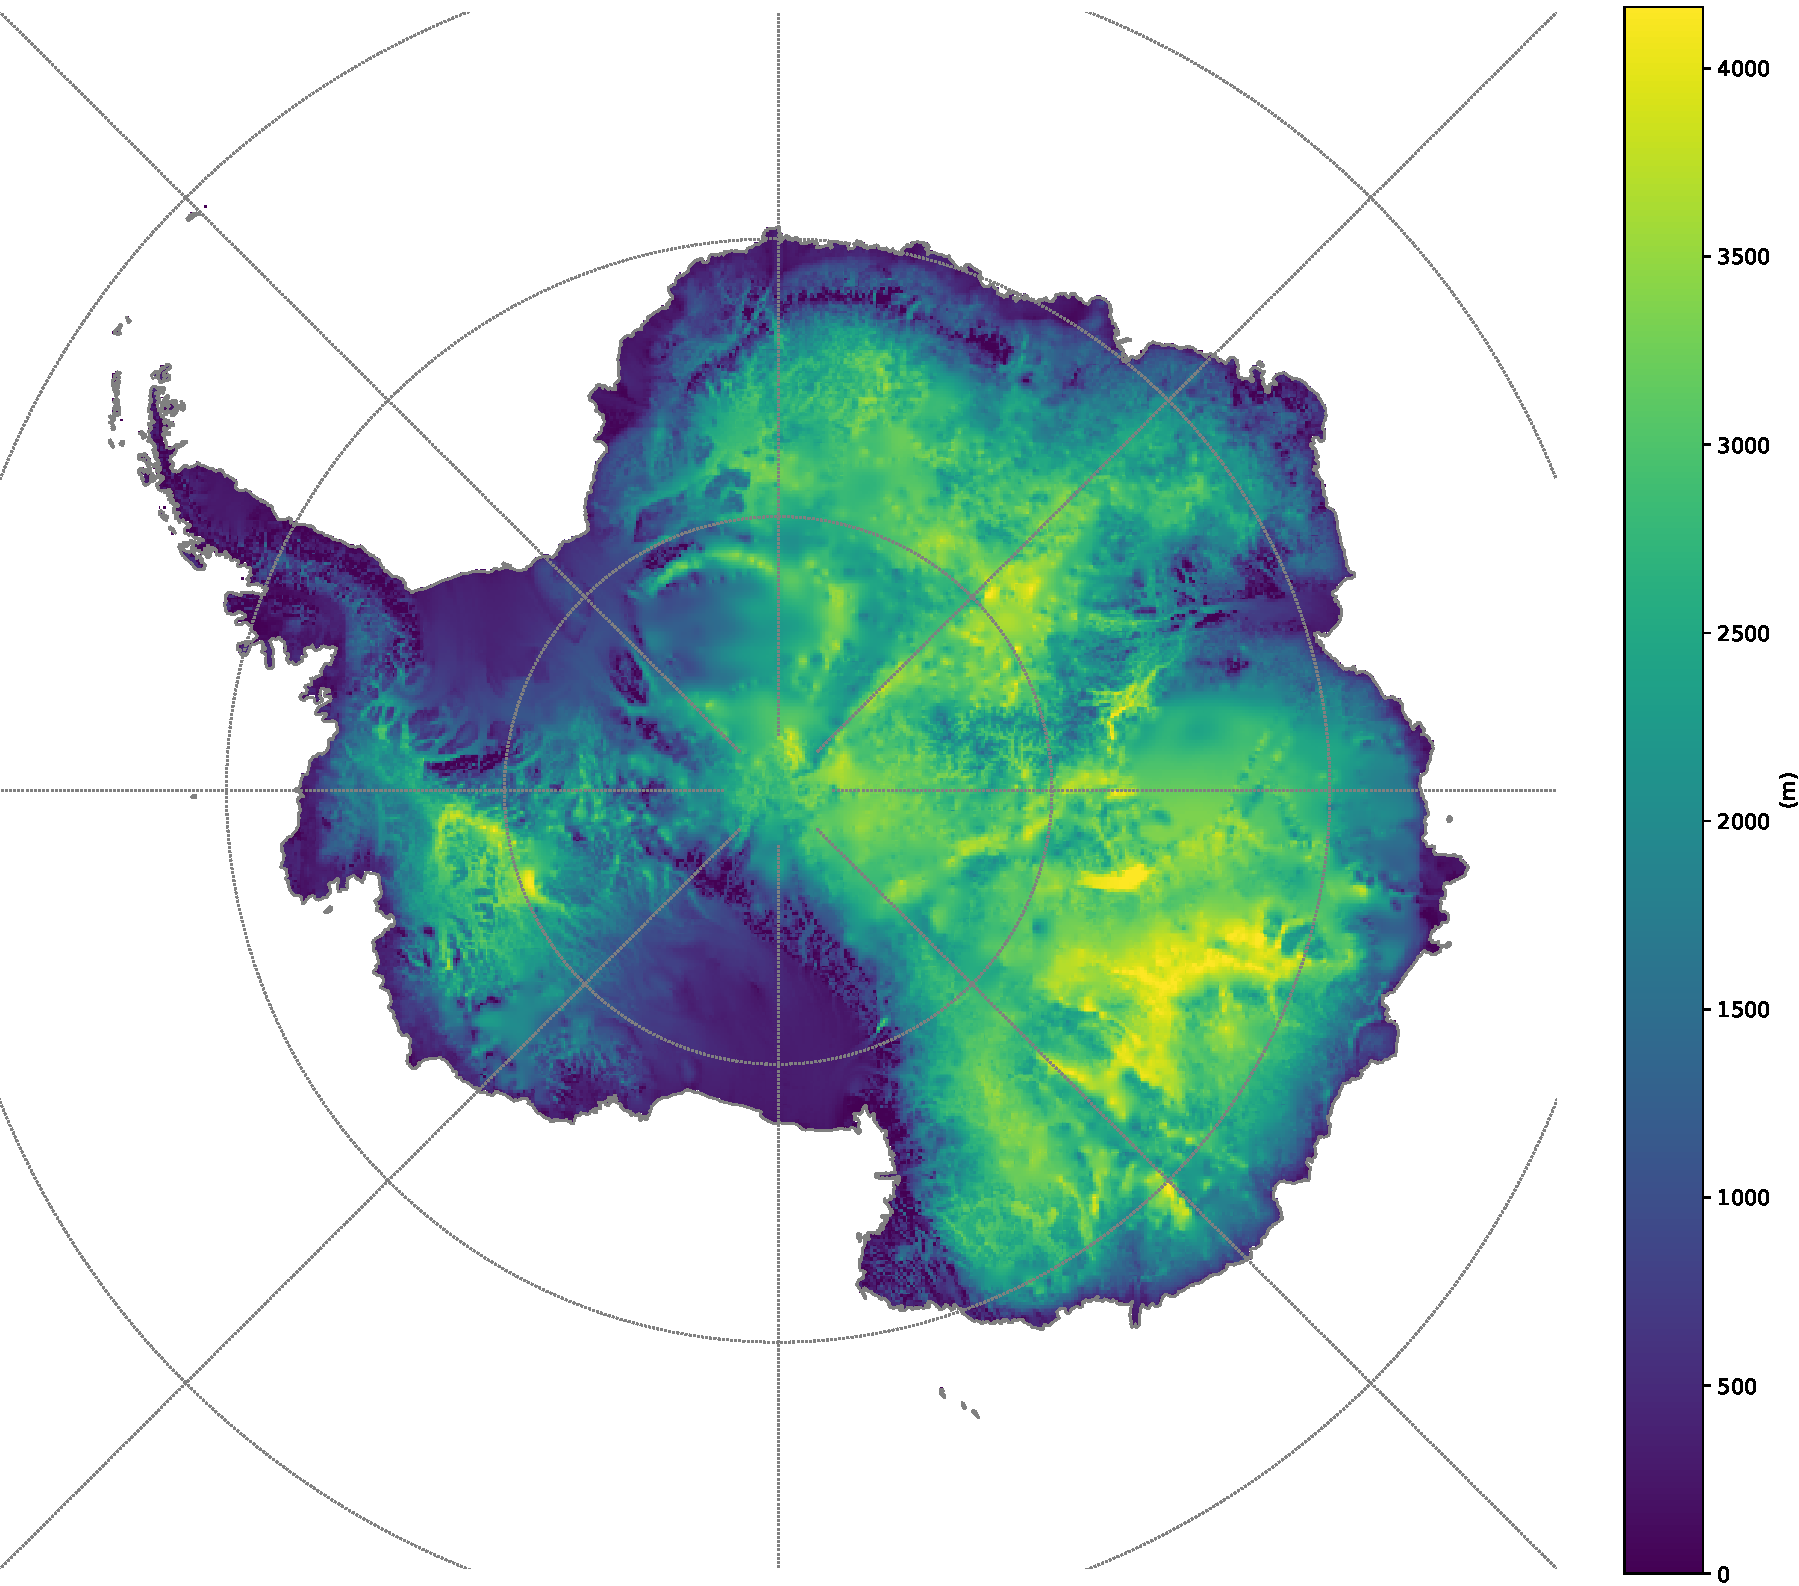
\includegraphics[height=10cm] {../fig/ice}};
	\end{scope}

	\begin{scope}[shift={(10,0)}]
		\node [anchor=south west] (seis) at (0,0) {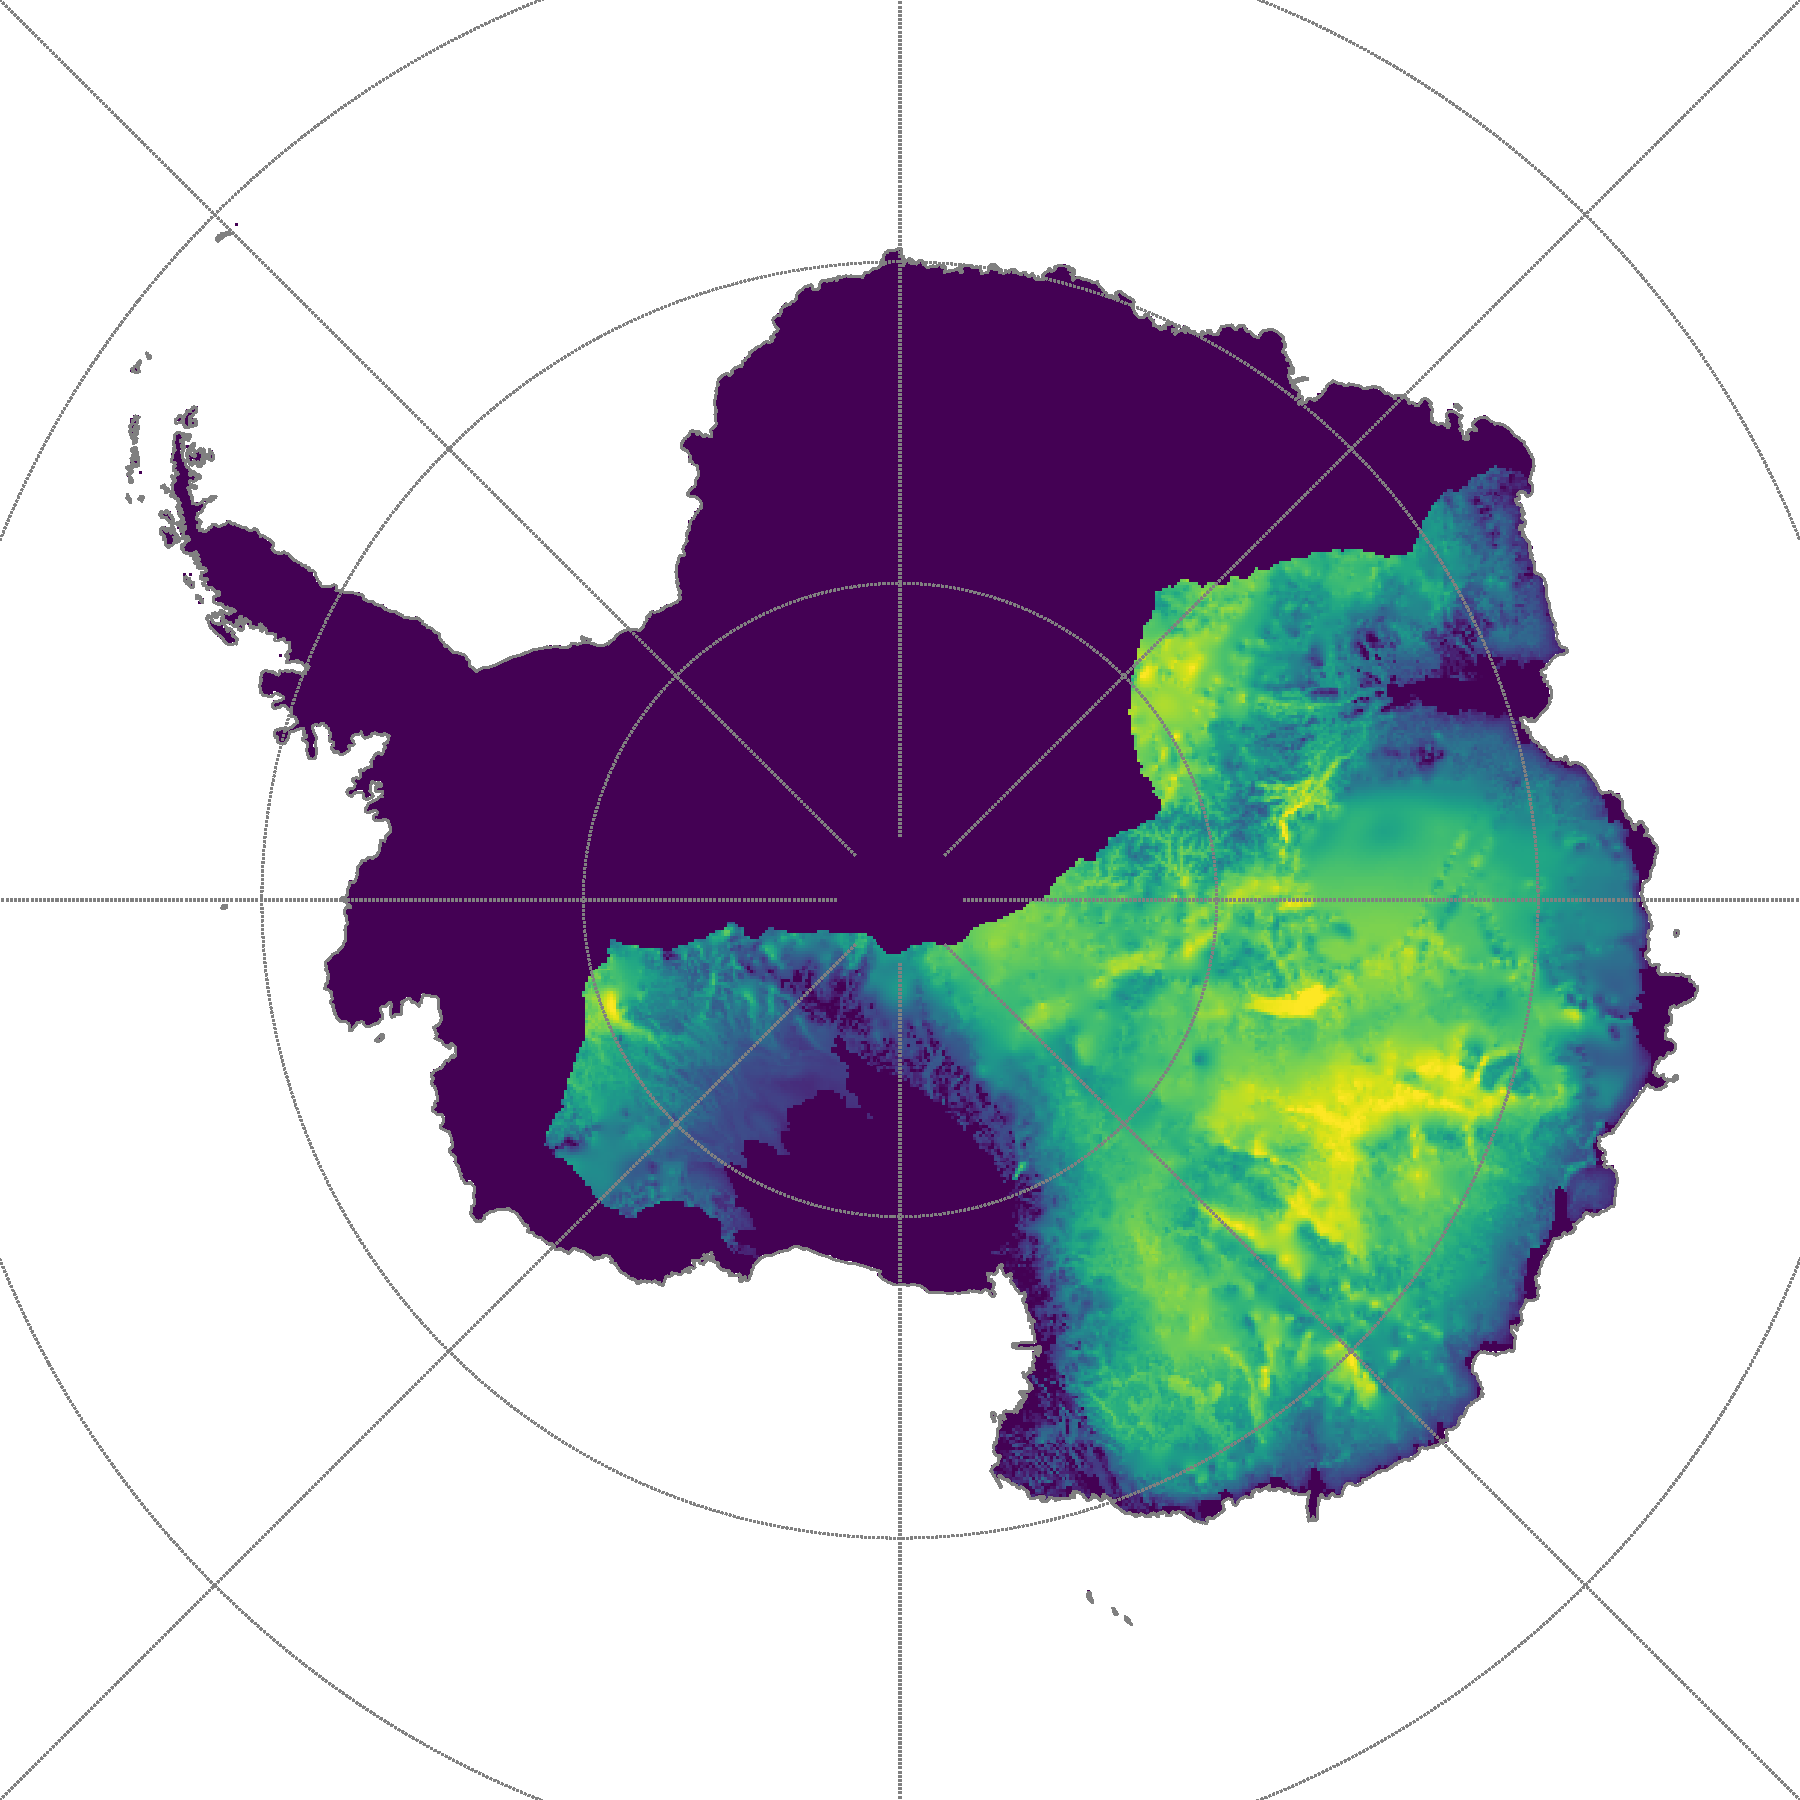
\includegraphics[height=10cm] {../fig/selected}};
	\end{scope}

	
	\begin{scope}[shift={(0,10)}]
		\node [anchor=south west] (seis) at (0,0) {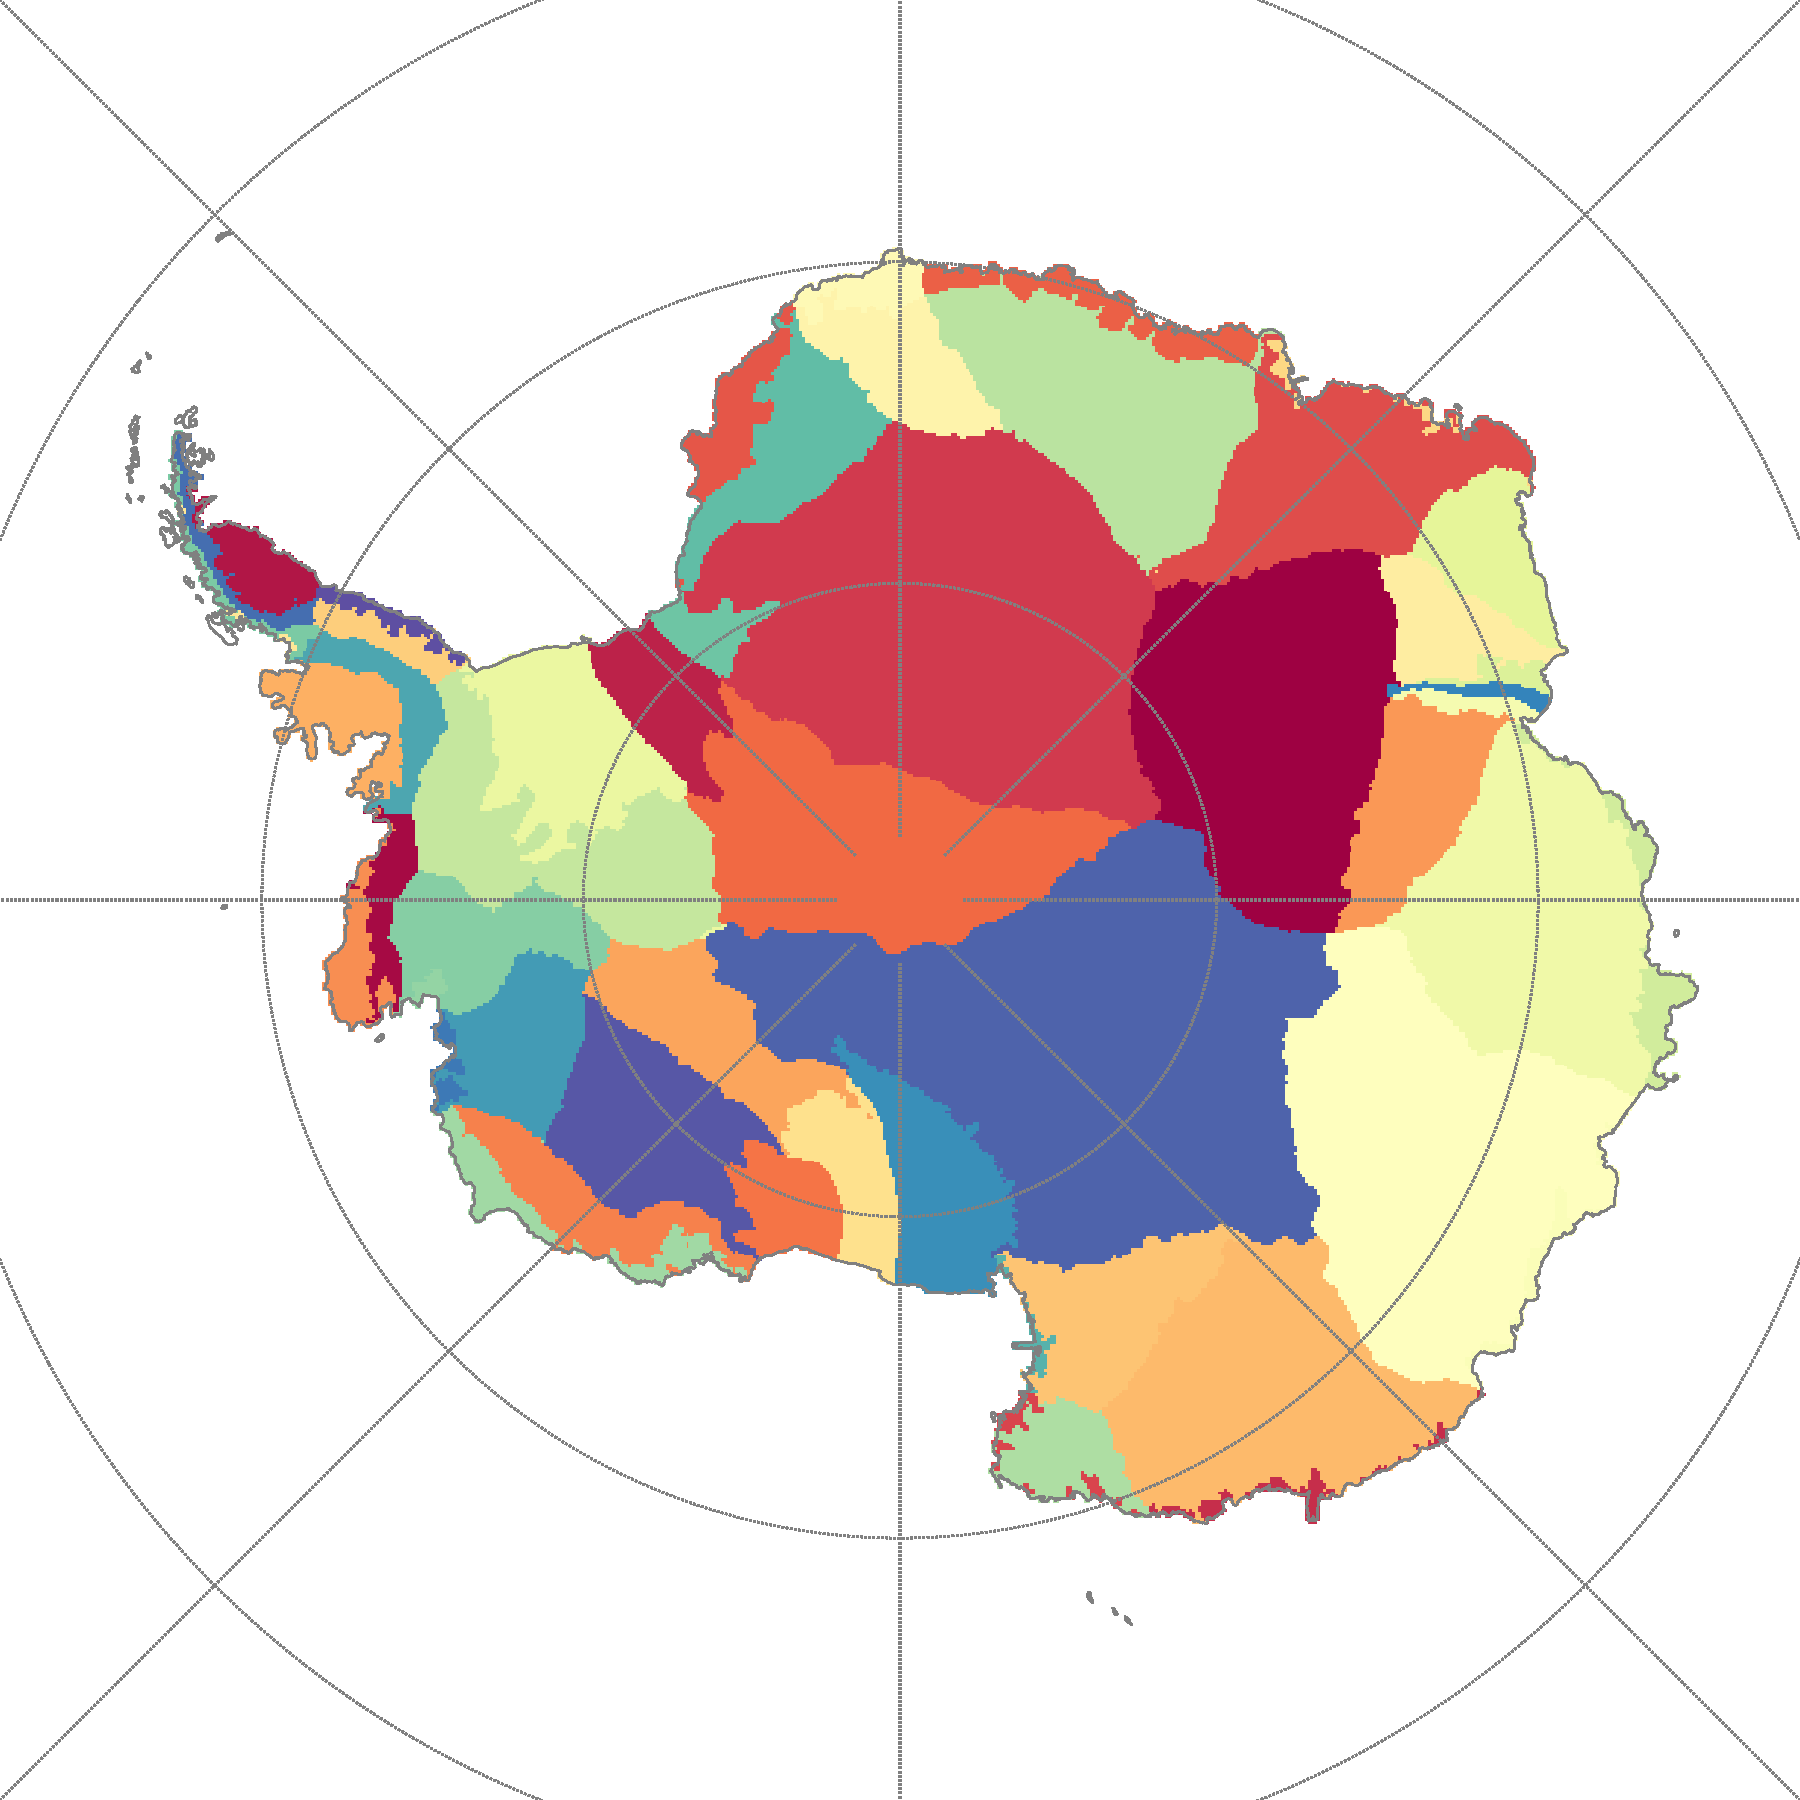
\includegraphics[height=10cm] {../fig/dranage}};
	\end{scope}


	\end{tikzpicture}
\end{figure}
\end{document}